\chapter{\textsc{Assembleur}}

On appelle \textit{langage machine} le langage natif du CPU, c'est à dire le langage qui peut être directement \textit{interprété} par le processeur. Les instructions sont des mots binaires organisés en champs, qui commandent chacun des actions spécifiques telles que :
\begin{itemize}[label=\textbullet,font=\small]
\item le type d'opération à effectuer
\item les opérandes
\item le mode d'adressage
\end{itemize}
Le langage machine est donc intrinsèquement lié au CPU auquel il s'applique,

Le langage d'assemblage (ou langage assembleur ou simplement assembleur par abus de
langage, abrégé ASM) est une version lisible du langage machine. Il consiste à représenter les codes binaires des instructions par des symboles appelés mnémoniques (du grec mnêmonikos, relatif à la mémoire), c'est-à-dire faciles à retenir.

Par exemple, l'unité de contrôle d'un processeur particulier reconnaît l'instruction en langage
machine suivante :

%MOV R0,#data	0x78
%\begin{tabbing}
%\qquad 01111000 01010101 b en binaire\\
%\qquad 0x78 0x55 en hexadécimal
%\end{tabbing}

\lstset{style=customc}
\begin{lstlisting}
01000000 00110101 00000000 01010101 b (en binaire)
4035 0055 h (en hexadécimal)
\end{lstlisting}

On voit bien qu'il est impossible de comprendre directement ce que peut faire cette instruction.
En langage assembleur, cette instruction est traduite par un équivalent plus facile à comprendre
pour le programmeur :
\lstset{style=customc}
\begin{lstlisting}
      MOV.W #85,R5
\end{lstlisting}

qui signifie "mettre la valeur décimale 85" (0x55 en hexadécimal) dans le registre R5.

\section{Jeu d'instructions}
Le jeu d'instructions est l'ensemble de toutes les instructions que le CPU est capable d'exécuter. On peut en général les regrouper en plusieurs catégories:
\begin{itemize}[label=\textbullet,font=\small]
\item instructions de transfert de données; elles consistent à copier le contenu d'un registre ou d'une case mémoire vers un autre registre ou une autre cas mémoire.
\item opérations arithmétiques;
\item opérations logiques;
\item sauts et rupture de séquence contrôlés ou non par un test, qui permettent (par exemple) de faire des appels de sous-programme.
\end{itemize}

En plus de cette classification, les instructions peuvent être à un ou deux opérandes. Dans les machines simples, jusqu'à 16-bits, les instructions à deux opérandes sont en général de la forme:
\lstset{style=customc}
\begin{lstlisting}
OP SRC DST
\end{lstlisting}
Le résultat de l'opération écrase l'un des opérandes.

\bigskip
Le jeu d'instruction d'un CPU peut être plus ou moins complet selon la complexité du CPU. Par exemple, celui de la famille MCS-51 (famille de microcontrôleurs Intel 8051 et 8052) comprend environ 110 instructions, alors que le MSP430 a "seulement" 27 instructions, tout en offrant des performances comparables.
Une raison est liée au \textit{mode d'adressage}, qui définit la façon dont le CPU accède aux données qu'il s'apprête à traiter, que ce soit pour un simple transfert de données ou une opération arithmétique sophistiquée.

\section{Modes d'adressage}
Selon que l'opérande d'une instruction est une constante, une variable, un pointeur ou autre, il est évident que cet opérande n'est pas identifié de la même manière.
Reprenant l'instruction prise comme exemple dans l'introduction:
\lstset{style=customc}
\begin{lstlisting}
      MOV.W #85,R5
\end{lstlisting}

la valeur "85", qui était codée par "0055" pourrait représenter:
\begin{itemize}[label=\textbullet,font=\small]
\item le nombre (la constante) 0x55 (ou 85 en décimal);
\item la case mémoire numéro 0x55;
\item si c'est la case mémoire numéro 0x55, est-ce son contenu qui est l'opérande ou autre chose ?
\item etc...
\end{itemize}

Même si les modes d'adressage varient grandement d'un CPU à un autre, on peut en identifier quelques uns qui leurs sont communs. Ce sont:
\begin{itemize}[label=\textbullet,font=\small]
\item l'adressage immédiat;
\item l'adressage direct;
\item l'adressage indirect;
\item l'adressage relatif;
\item l'adressage indexé.
\end{itemize}

D'autres modes d'adressage sont imaginables selon le type de machine.

\subsection{Adressage immédiat}
En adressage \textit{immédiat}, la donnée est identifiée explicitement. Dans l'exemple déjà vu 
\lstset{style=customc}
\begin{lstlisting}
      MOV.W #85,R5
\end{lstlisting}

le symbole \# spécifie que la valeur est à prendre telle quelle.
L'adressage immédiat est donc associé à une constante.

\subsection{Adressage direct}
En adressage \textit{direct}, parfois aussi appelé \textit{absolu}, l'identifiant est l'adresse de la case contenant la donnée. L'exemple devient
\lstset{style=customc}
\begin{lstlisting}
      MOV.W 85,R5
\end{lstlisting}
C'est l'adressage "par défaut", le plus courant, spécifié par le symbole \& ou par l'absence de symbole. L'adressage direct est donc associé à une variable. De fait, la case mémoire ou le registre identifié est une variable.

\subsection{Adressage indirect}
En adressage \textit{indirect}, l'identifiant est l'adresse d'une case mémoire, qui contient l'adresse de la donnée visée . L'exemple devient
\lstset{style=customc}
\begin{lstlisting}
      MOV.W @85,R5
\end{lstlisting}
Cet adressage est souvent spécifié par le symbole @. L'adressage indirect permet donc d'implémenter un pointeur.

\subsection{Adressage relatif}
Le terme "adressage" est ici abusif dans la mesure où l'adressage relatif est utilisé pour faire des sauts et branchements. L'adresse est ici celle d'une instruction. L'adressage relatif spécifie l'adresse de la prochaine instruction sous forme d'un saut par rapport à la position de l'instruction en cours d'exécution.
En pratique, il n'y a pas à se soucier du calcul du déplacement pour faire le saut au bon endroit; c'est le logiciel de développement qui se charge de calculer la bonne valeur.
Un exemple d'instruction avec adressage relatif est:
\lstset{style=customc}
\begin{lstlisting}
      JMP Label
\end{lstlisting}

{\fontfamily{pcr}\selectfont Label} est une \textit{étiquette} permettant de repérer la prochaine instruction, par exemple:
\lstset{style=customc}
\begin{lstlisting}
Label	MOV.W @85,R5
\end{lstlisting}
L'exécution de l'instruction {\fontfamily{pcr}\selectfont JMP Label} fait que la prochaine instruction est {\fontfamily{pcr}\selectfont MOV.W @85,R5} quel que soit l'endroit du programme où se trouve cette dernière.

\subsection{Adressage indexé}
L'adressage \textit{indexé} permet de gérer des tableaux de façon efficace. Il est le plus souvent associé à de l'adressage direct ou indirect. L'index permet d'accéder à plusieurs opérandes successifs à partir d'une position de départ.

\subsection{Adressage par registre}
Comme nous le verrons dans le chapitre suivant, le coeur du CPU contient des registres à usage général et à accès rapide, permettant de minimiser le temps d'exécution de certaines instructions. Ces registres sont identifiés explicitement, par un nom symbolique (par exemple A, ACC, R0, R1, R2, etc...).
Parfois appelé adressage \textit{implicite} ou \textit{inhérent}, le mode d'adressage par registre utilise donc explicitement le nom du registre impliqué. Par exemple:
\lstset{style=customc}
\begin{lstlisting}
      MOV R1,0x40
\end{lstlisting}
est une instruction du jeu d'instruction MCS-51 (microcontrôleurs de la famille 8051) et qui consiste à copier le contenu de la case d'adresse 0x40 (adressage direct pour la source de la donnée) dans le registre appelé R1. Bien que R1 pourrait être identifié par son adresse, il l'est ici par son nom explicite. L'intérêt est de pouvoir représenter le code de l'instruction sur moins d'octets que si l'adresse de R1 devait être fournie.

L'exemple suivant (toujours du jeu d'instruction MCS-51) utilise de l'adressage indirect par registre et de l'adressage avec un registre particulier appelé \textit{accumulateur}:
\lstset{style=customc}
\begin{lstlisting}
      MOV A,@R2
\end{lstlisting}

\subsection{Orthogonalité du jeu d'instruction}
Le jeu d'instruction d'un CPU est dit orthogonal lorsque tous les modes d'adressage disponibles sont utilisables avec toutes les instructions, pour autant que le mode d'adressage considéré a du sens avec l'instruction considérée.

\section{Jeu d'instruction du MSP430}
Les chapitres suivants donnent les modes d'adressage disponibles, et des exemples d'instructions du MSP430 pour chaque mode d'adressage. La liste exhaustive peut être consultée dans le manuel d'utilisateur de la famille MSP430 (document SLAU208, pages 185 à 340).

\subsection{Modes d'adressage}
L'espace mémoire complet est adressable sans exception. Toutefois, les modes d'adressage disponibles sont différents pour l'opérande source et l'opérande destination:
\begin{itemize}[label=\textbullet,font=\small]
\item sept modes d'adressage pour les opérandes de source
\item quatre modes d'adressage pour les opérandes de destination
\end{itemize}

Ces modes d'adressage sont applicables aussi bien à des instructions de transfert de données(MOV) qu'à des opérations arithmétiques (ADD, SUB,...).
La table \ref{table:MSP430_Addr_Reg} donne les différents modes d'adressage. Les champs \textit{Ad} (destination) et \textit{As} (source) définissent le mode pour chaque opérande et font partie du code de l'instruction. 
\begin{table}[H]
\centering 
\begin{tabular}{l c l l l l l}
\hline\hline
As & Ad & & Mode & & Syntaxe & Description \\ %[0.5ex]
\hline
00 & 0 & & Registre & & Rn & Les opérandes sont les contenus des registres  \\
01 & 1 & & Indexé & & x(Rn) & [Rn+x] pointe l'opérande. Les instructions utilisant ce mode\\
& & & & & & d'adressage contiennent au moins deux mots. Le second contient x \\
01 & 1 & & Symbolique & & Adresse & [PC+x] pointe l'opérande. Il s'agit d'un mode indexé x(PC)\\
& & & & & & Les instructions utilisant ce mode d'adressage contiennent\\
& & & & & &  au moins deux mots. Le second contient x \\
01 & 1 & & Direct (Absolu) & & \&Adresse & Le ou les deux mots de 16 bits suivant l'instruction contiennent les\\
& & & & & & valeurs des adresses. Le mode utilisé est le mode indexé x(SR) \\
10 & - & & Indirect & & @Rn & [Rn] pointe l'opérande \\
11 & - & & Indirect avec & & @Rn+ & [Rn] pointe l'opérande puis Rn+1 -> Rn\\
& & & autoincrément & & & Il y a donc post-incrémentation \\
11 & - & & Immédiat & & $\#N$ & Les instructions utilisant ce mode d'adressage contiennent\\
& & & & & & au moins deux mots. Le second contient N \\
& & & & & & Il s'agit d'un mode avec auto-incrémentation\\
& & & & & & PC+1 -> PC puis [PC] pointe N \\
\hline
\end{tabular}
\caption{Modes d'adressage du MSP430}
\label{table:MSP430_Addr_Reg}
\end{table}

Les modes \textit{indexé}, \textit{symbolique} et \textit{direct} sont considérés comme trois cas particuliers du mode \textit{indexé}. Le mode \textit{direct} considère l'adresse comme un index à ajouter à l'adresse 0x0000. Le mode \textit{symbolique} considère l'adresse comme un index à ajouter au compteur de programme PC.

\subsection{Format des instructions}
Les instructions sont en principe codées sur un mot de 16 bits, auquel s'ajoutent éventuellement 1 ou 2 mots selon le mode d'adressage utilisé. Par exemple, l'adressage immédiat nécessite de joindre le ou les opérandes au code de l'instruction.

Pour le codage de l'instruction elle-même, il existe trois formats selon le nombre d'opérandes:
\begin{itemize}[label=\textbullet,font=\small]
\item format I pour les instructions à 2 opérandes. Par exemple, une addition exécute une opération du type\\ $SRC + DST -> DST$ (source + destination va dans destination)
\item format II pour les instructions à 1 opérandes;
\item format III, spécifique pour les instructions de test et branchement.
\end{itemize}

les figures \ref{fig:Inst_format_1}, \ref{fig:Inst_format_2} et \ref{fig:Inst_format_jump} illustrent comment sont structurées les instructions selon leur format.

\begin{figure}[htb]
  \centering
  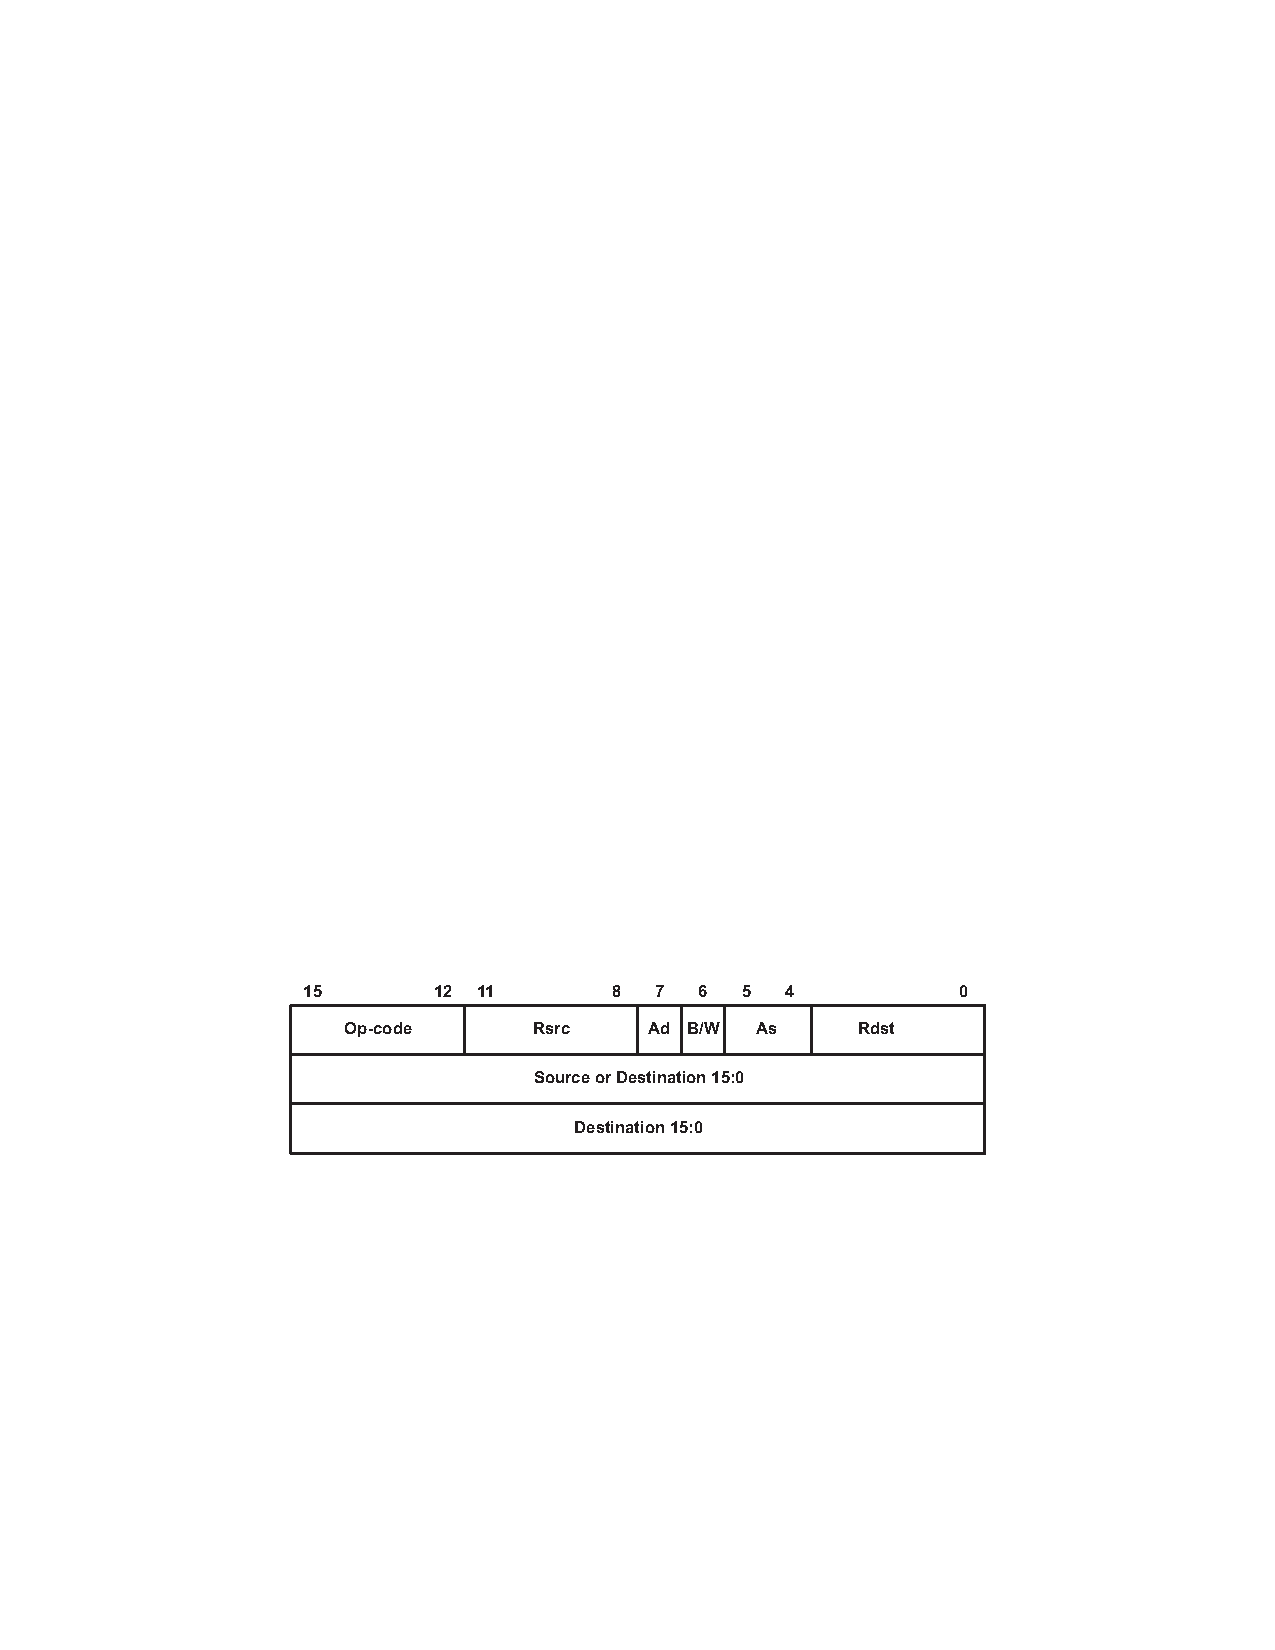
\includegraphics[angle=0, width=14cm]{./Figures/Assembleur/Inst_format_1.pdf}
  \rule{35em}{0.5pt}
  \caption[Schéma Timer]{Format I des instructions à deux opérandes}
  \label{fig:Inst_format_1}
\end{figure}

\begin{figure}[htb]
  \centering
  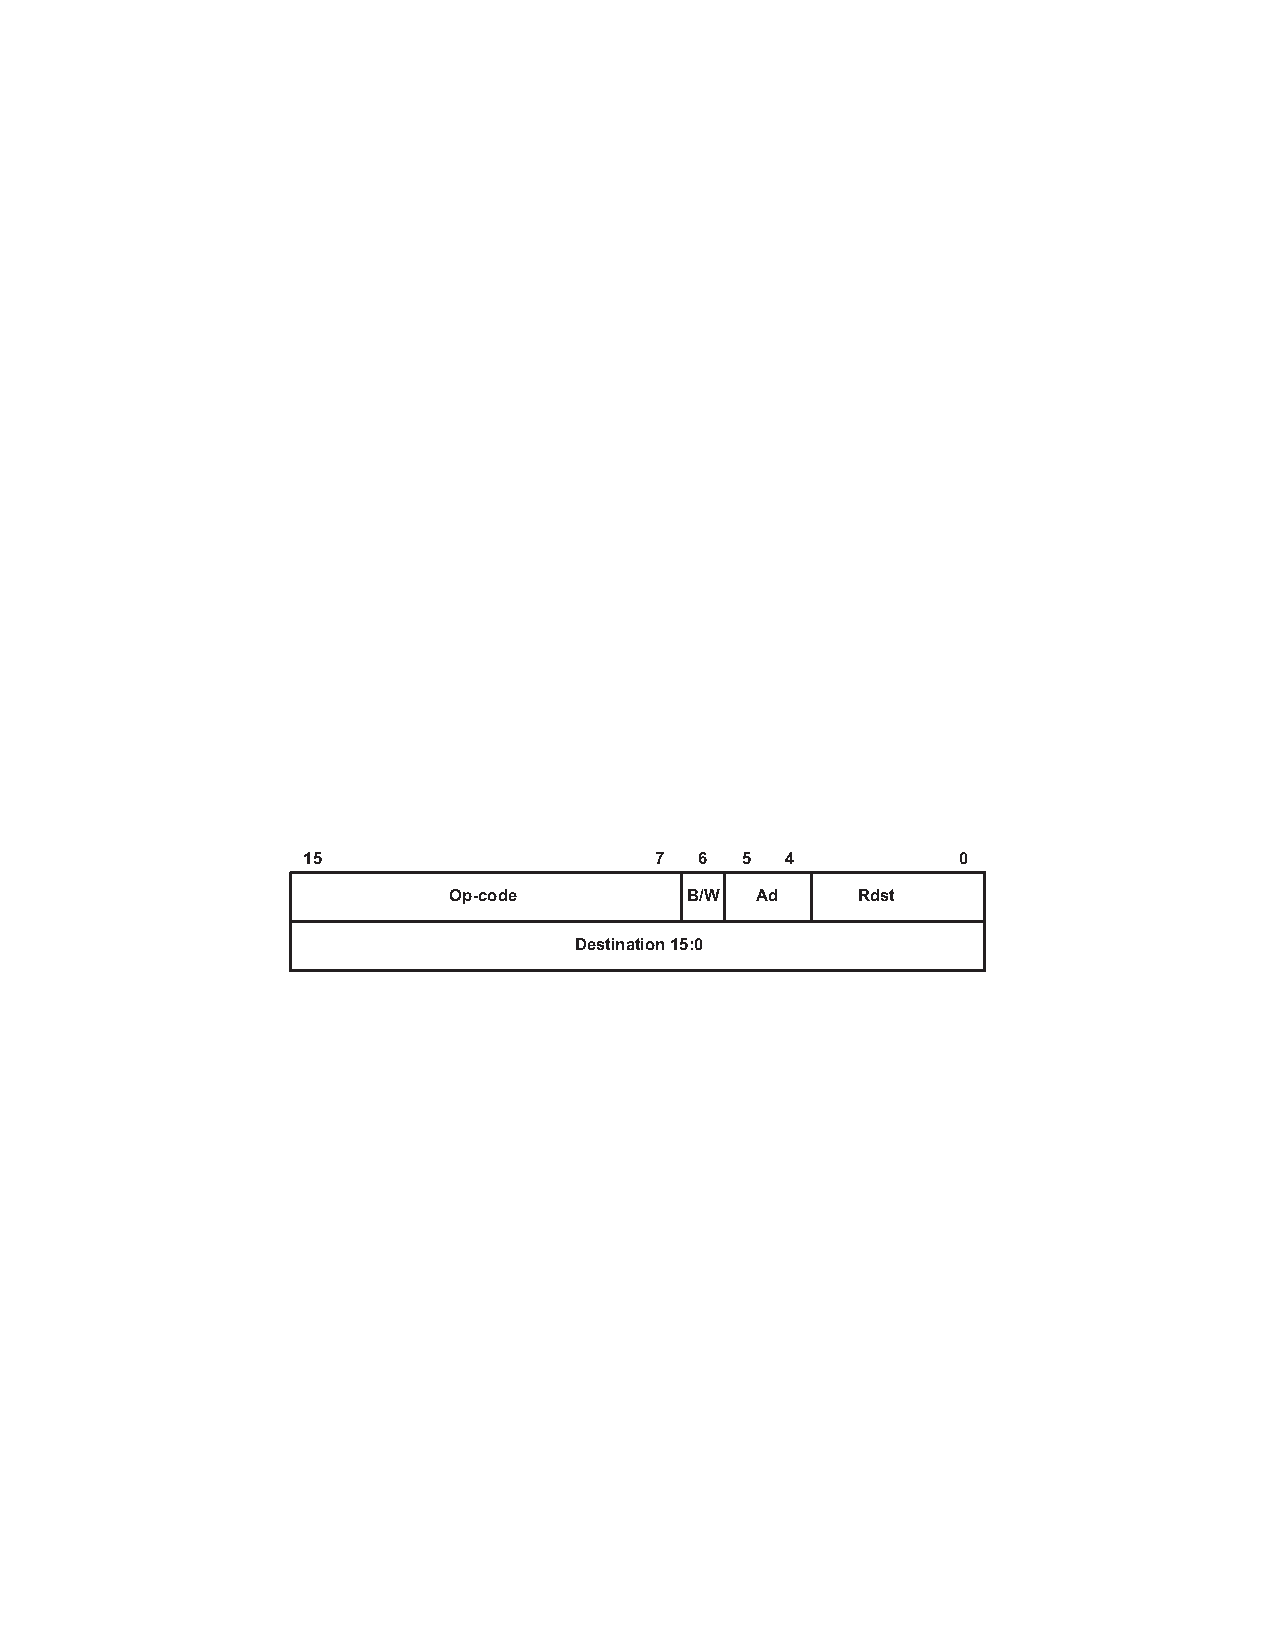
\includegraphics[angle=0, width=14cm]{./Figures/Assembleur/Inst_format_2.pdf}
  \rule{35em}{0.5pt}
  \caption[Schéma Timer]{Format II des instructions à un opérande}
  \label{fig:Inst_format_2}
\end{figure}

\begin{figure}[htb]
  \centering
  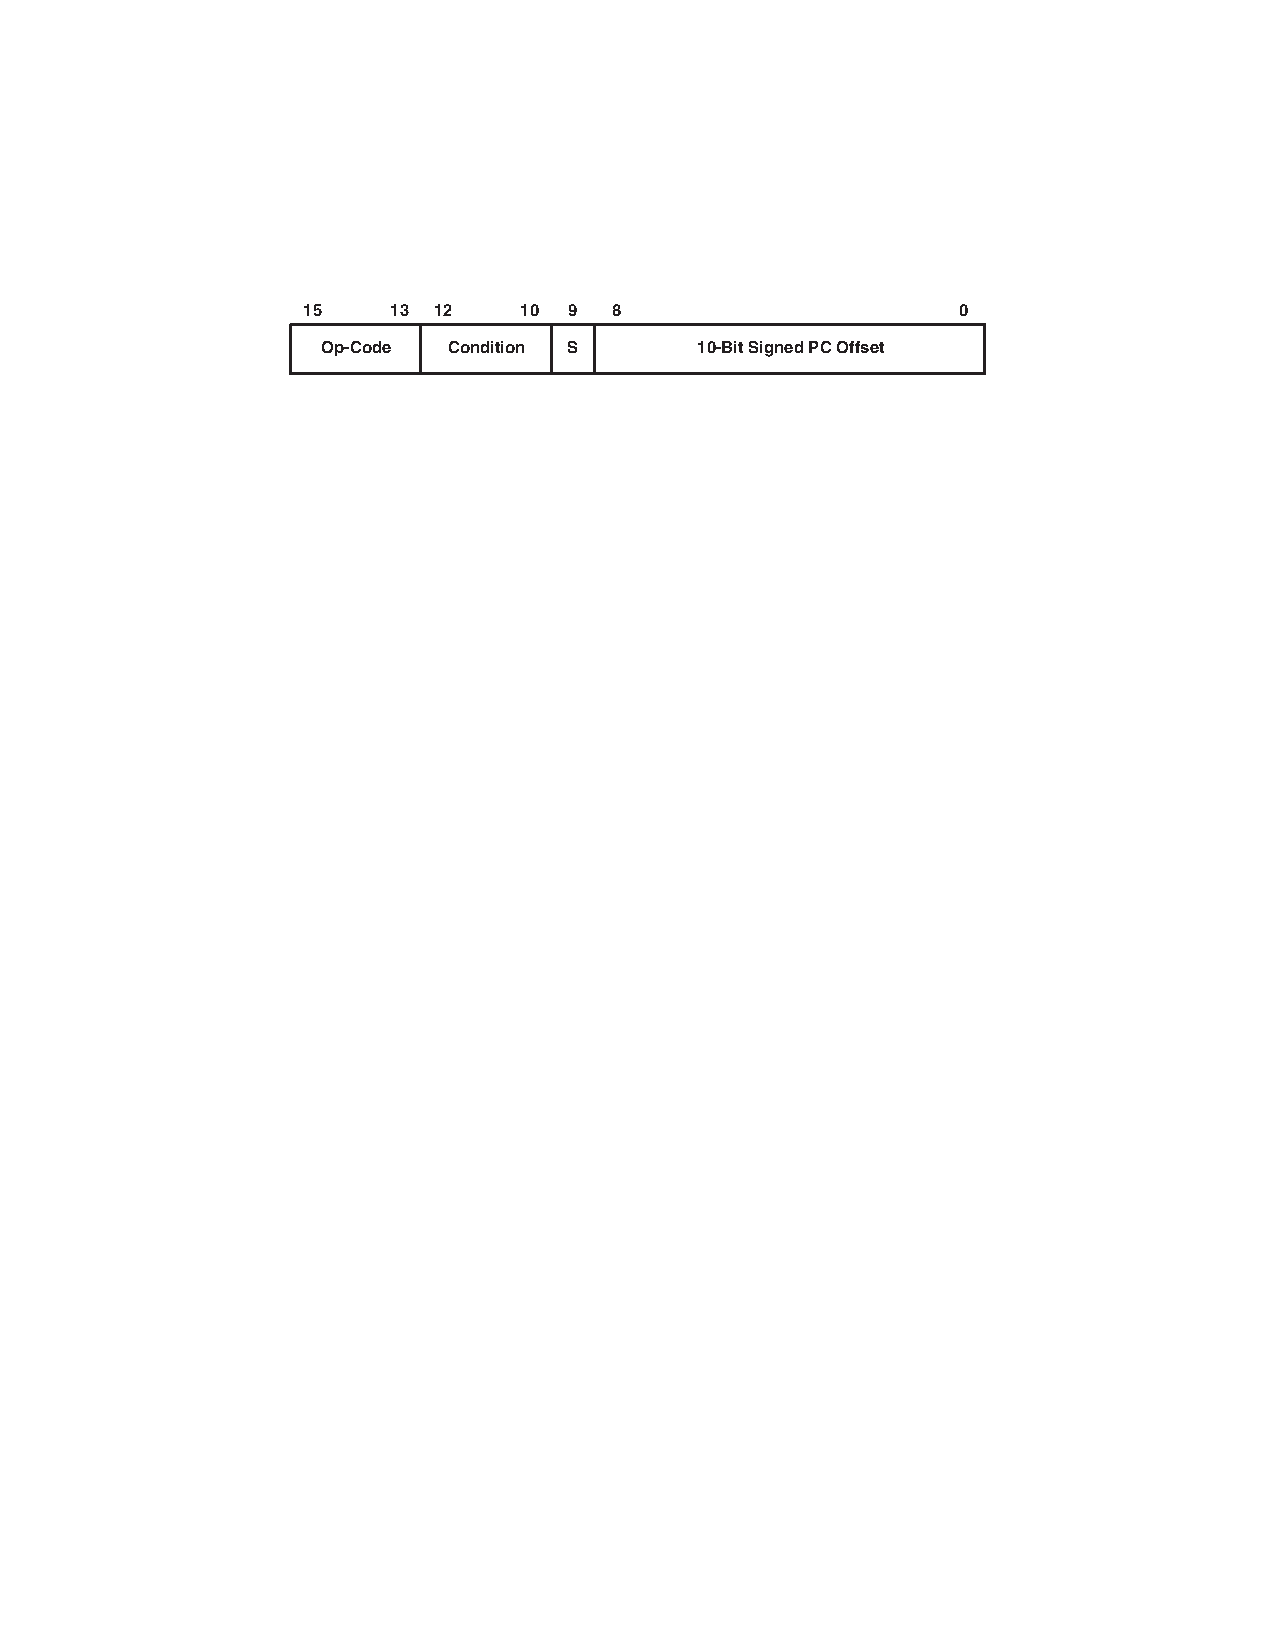
\includegraphics[angle=0, width=14cm]{./Figures/Assembleur/Inst_format_jump.pdf}
  \rule{35em}{0.5pt}
  \caption[Schéma Timer]{Format III pour instructions de test et branchement}
  \label{fig:Inst_format_jump}
\end{figure}

\pagebreak
\subsection{Exemple 1: adressage par registre}
Le CPU MSP430 contient 16 registres notés R0 à R15. Chacun d'entre eux peut être utilisé avec ce mode d'adressage. L'instruction
\lstset{style=customc}
\begin{lstlisting}
      MOV.W R10,R8
\end{lstlisting}
permet de copier le contenu du registre R10 dans le registre R8. Le suffixe \textit{.W} spécifie que les opérandes sont des mots (de 16 bits).
L'instruction est codée sur un mot de 16 bits et utilise le format I, comme indiqué dans la figure \ref{fig:Inst_format_1}. Du fait que l'adressage est \textit{par registre}, cette instruction n'a pas besoin d'autres informations que l'identification des registres R10 et R8.
Son code est:
\lstset{style=customc}
\begin{lstlisting}
Instruction: 0100 1010 0000 1000 ou 0x4A08
\end{lstlisting}

Op-code = 4, Rsrc = 10, Ad=0, B/W=0, As=0, Rdst=8

\subsection{Exemple 2: adressage indexé par registre}
L'adressage indexé du MSP430 est en fait un adressage indirect indexé. En effet, le contenu du registre considéré est additionné à l'index pour obtenir l'adresse de l'opérande. L'instruction
\lstset{style=customc}
\begin{lstlisting}
      MOV.B R10,5(R8)
\end{lstlisting}
permet de copier le contenu du registre R10 dans la case mémoire dont l'adresse est égale à 5 plus le contenu du registre R8. Le suffixe \textit{.B} spécifie que les opérandes sont des octets.
L'instruction utilise le format I, et est codée sur deux mots de 16 bits; un pour l'instruction elle-même, l'autre est égal à 5.
Son code est:
\lstset{style=customc}
\begin{lstlisting}
Premier mot: 0101 1010 1100 1000   ou 0x4AC8
Second mot : 0000 0000 0000 0101   ou 0x0005
\end{lstlisting}

Op-code = 4, Rsrc = 10, Ad=1, B/W=1, As=0, Rdst=8

\subsection{Exemple 3: adressage direct}
L'instruction
\lstset{style=customc}
\begin{lstlisting}
      ADD.W   R10,&3310
\end{lstlisting}
permet d'additionner le contenu du registre R10 à celui de la case mémoire d'adresse 3310 et de placer le résultat dans cette case mémoire.
L'instruction utilise le format I, et est codée sur deux mots de 16 bits; un pour l'instruction elle-même, l'autre est égal à 0x0CEE (3310 en décimal).
Son code est:
\lstset{style=customc}
\begin{lstlisting}
Premier mot: 0101 1010 1000 0010   ou 0x5A82
Second mot : 0000 1100 1110 1110   ou 0x0CEE
\end{lstlisting}

Op-code = 5, Rsrc = 10, Ad=1, B/W=0, As=0, Rdst=2
Comme indiqué dans la table \ref{table:MSP430_Addr_Reg}, cet adressage est considéré comme de l'adressage indexé. Le registre R2 est ici utilisé comme générateur de l'adresse de départ 0x0000.

\subsection{Exemple 4: adressage indirect}
L'instruction
\lstset{style=customc}
\begin{lstlisting}
      ADD.W   @R10,R8
\end{lstlisting}
permet d'additionner le contenu de la case mémoire dont l'adresse est dans le registre R10 au contenu de R8 et de placer le résultat dans R8.
L'instruction utilise le format I, et est codée sur un mot de 16 bits.
Son code est:
\lstset{style=customc}
\begin{lstlisting}
Instruction: 0101 1010 0010 1000 ou 0x5A28
\end{lstlisting}

Op-code = 5, Rsrc = 10, Ad=0, B/W=0, As=2, Rdst=8

\subsection{Exemple 5: adressage indirect avec autoincrément}
L'instruction
\lstset{style=customc}
\begin{lstlisting}
      ADD.W   @R10+,R8
\end{lstlisting}
permet d'additionner le contenu de la case mémoire dont l'adresse est dans le registre R10 au contenu de R8 et de placer le résultat dans R8. A la fin de cette instruction, le contenu de R10 est incrémenté de 2 unités pour pointer sur le prochain mot. Il serait incrémenté de 1 si le suffixe \textit{.B} avait été utilisé.
L'instruction utilise le format I, et est codée sur un mot de 16 bits.
Son code est:
\lstset{style=customc}
\begin{lstlisting}
Instruction: 0101 1010 0011 1000 ou 0x5A38
\end{lstlisting}

Op-code = 5, Rsrc = 10, Ad=1, B/W=0, As=3, Rdst=8

\subsection{Exemple 6: adressage immédiat}
L'instruction
\lstset{style=customc}
\begin{lstlisting}
      ADD.W   #3253,&3310
\end{lstlisting}
permet d'additionner la valeur 3253 (décimal) au contenu de la case mémoire d'adresse 3310 et de placer le résultat dans cette case mémoire.
L'instruction utilise le format I, et est codée sur trois mots de 16 bits; un pour l'instruction elle-même, le second pour la valeur 3253, le troisième est égal à 0x0CEE (3310 en décimal).
Son code est:
\lstset{style=customc}
\begin{lstlisting}
Premier mot   : 0101 1010 1000 0010	ou 0x50B2
Second mot    : 0000 1100 1011 0101 ou 0x0CB5 (3253 en décimal)
Troisième mot : 0000 1100 1110 1110 ou 0x0CEE
\end{lstlisting}

Op-code = 5, Rsrc = 00, Ad=1, B/W=0, As=0, Rdst=2

\subsection{Exemple 7: adressage symbolique}
L'instruction
\lstset{style=customc}
\begin{lstlisting}
      CALL   #routine
\end{lstlisting}
permet "d'envoyer" le CPU exécuter l'instruction située à l'adresse {\fontfamily{pcr}\selectfont routine}. Cette instruction sera de fait considérée comme la première du groupe qui suit, qui constitue donc un \textit{sous-programme}. La fin de ce sous-programme est délimitée par une instruction appelée {\fontfamily{pcr}\selectfont RET}.
L'instruction donnée en exemple utilise le format II, et est codée sur deux mots de 16 bits; un pour l'instruction elle-même, le second pour l'adresse {\fontfamily{pcr}\selectfont routine}.
Si {\fontfamily{pcr}\selectfont routine = 0x31A2}, le code de l'instruction est:
\lstset{style=customc}
\begin{lstlisting}
Premier mot   : 0001 0010 1011 0000	ou 0x50B2
Second mot    : 0011 0001 1010 0010 ou 0x31A2 
\end{lstlisting}

Op-code = 0x25, B/W=0, Ad=3, Rdst=0

\subsection{Exemple 8: adressage symbolique}
L'instruction
\lstset{style=customc}
\begin{lstlisting}
      JMP   label
\end{lstlisting}
permet de faire un saut dans le programme, dans un sens ou dans l'autre, d'au maximum 1024 adresses, sans retour prévu.
L'instruction donnée en exemple utilise le format III, et est codée sur un mot de 16 bits.
Si {\fontfamily{pcr}\selectfont label = 0x31A8}, et si l'instruction est localisée à l'adresse 0x314E, alors le code de l'instruction est:
\lstset{style=customc}
\begin{lstlisting}
Instruction :  0011 1100 0010 1101	ou 0x3C2D
\end{lstlisting}
Le champ "PC Offset" (voir figure \ref{fig:Inst_format_jump}) est calculé de sorte que\\
$0x0314E + 2*PC\_Offset = 0x31A8 $

\section{Chaine de compilation}
Le développement d'un programme pour microcontrôleur consiste à générer du code machine à partir d'un programme écrit en C ou en C++, en passant par une vue en langage \textit{assembleur}.
En général, le processus de génération du code machine doit permettre de réutiliser du code déjà écrit, comme une librairie de fonctions que l'on aura déjà testées, validées et documentées. Une question se pose alors, qui est le calcul des adresses de début de ces fonctions. Ce calcul est réalisé lors d'une opération appelée \textit{édition de lien}.

la figure \ref{fig:develop_flow} illustre le processus de développement de code.
\begin{figure}[htb]
  \centering
  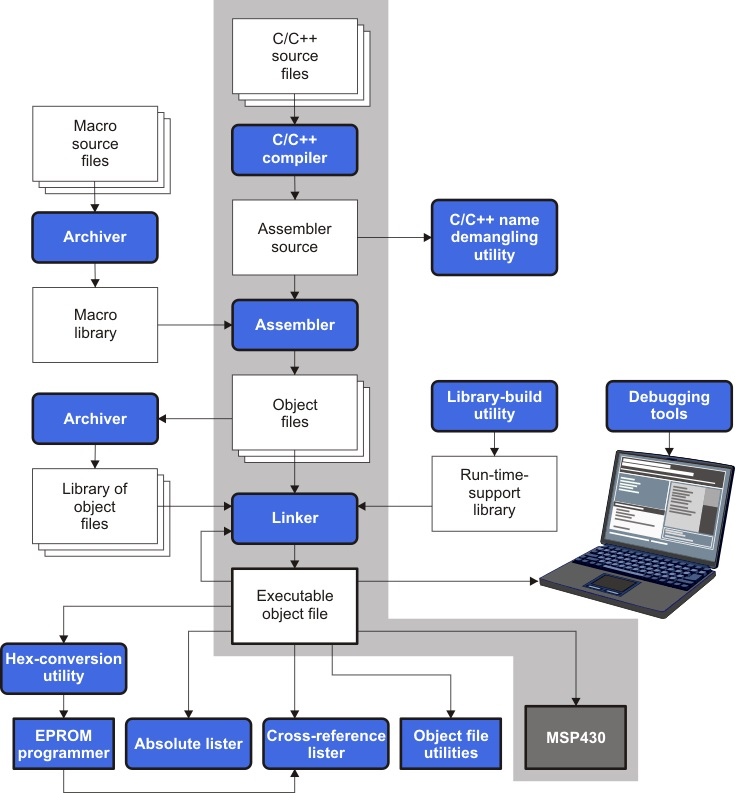
\includegraphics[angle=0, width=14cm]{./Figures/Assembleur/develop_flow.jpg}
  \rule{35em}{0.5pt}
  \caption[Schéma Timer]{Processus de développement de code}
  \label{fig:develop_flow}
\end{figure}

La partie grisée de la figure montre le chemin le plus courant pour le développement. Les autres parties sont optionnelles.\\

Le point d'entrée du processus (haut de la figure) est le code source, écrit en langage C ou C++.\\

La première étape est la compilation, qui traduit le code source en langage assembleur. Dans l'outil de développement, il est possible de voir le code assembleur correspondant au code source.
A ce stade, la localisation du code assembleur dans la mémoire est provisoire, puisqu'il faut encore tenir compte des fonctions déjà existantes.\\

Dans la seconde étape, l'outil d'assemblage (appelé \textit{l'assembleur} transforme donc les fichiers en langage assembleur en fichiers \textit{objet} relocalisables. Cette étape implique de connaître en particulier les liens entre les instructions de type {\fontfamily{pcr}\selectfont JMP} et {\fontfamily{pcr}\selectfont CALL} et les instructions vers lequel elles pointent.\\

La troisième étape est l'édition de lien, qui consiste à combiner les fichiers relocalisables en un fichier exécutable (en langage machine) unique, dans lequel les adresses exactes de toutes les instructions sont fixées.\\

Une fois le fichier contenant le code exécutable obtenu, il peut être transféré dans la mémoire du microcontrôleur via un port spécifique appelé JTAG.  En général, le transfert s'effectue par une liaison USB. L'interface entre le port USB et le port JTAG offre des fonctionnalités de debug, telles que:
\begin{itemize}[label=\textbullet,font=\small]
\item possibilité de placer des points d'arrêt lors de l'exécution du code;
\item possibilité d'exécuter le programme pas à pas;
\item etc...
\end{itemize}
Pour cette raison, cette interface est souvent appelée \textit{sonde programmation et debug} ou \textit{sonde de debug} ou encore \textit{sonde JTAG}.
